\chapter{Experiment}
\label{ch:Experiment}
As has already been shown, the sealing of valves is essential for the reliability in hydraulic and pneumatic systems. Leakage can impact the efficiency
 of industrial production and contribute to the occurrence of potential dangers. 
Due to these factors, it is crucial to investigate leaks in metal valves. According to a search 
of the scholarly literature, there are limited discussions of the effect of particles in fluids 
and their concentration on the seal ability of metal valves. For the investigation of these 
factors' effects on the sealing of metal valves, the improvement of the test rig and the 
reasonable assessment of leakage under varying experimental settings are therefore imperative.

%%%%%%%%%%%%%%%%%%%%%%%%% new section: Test Rig
\section{Test Rig}
\label{Test Rig}

Figure \Ref{fig:oldTestRig} depicts a developed experimental platform that was available before this study 
was carried out. A ball seat valve, a water tank, pipelines, an air motor, a hydraulic pump,
and ball valves are its primary components.\\


\begin{figure}[htbp]
    \centering
    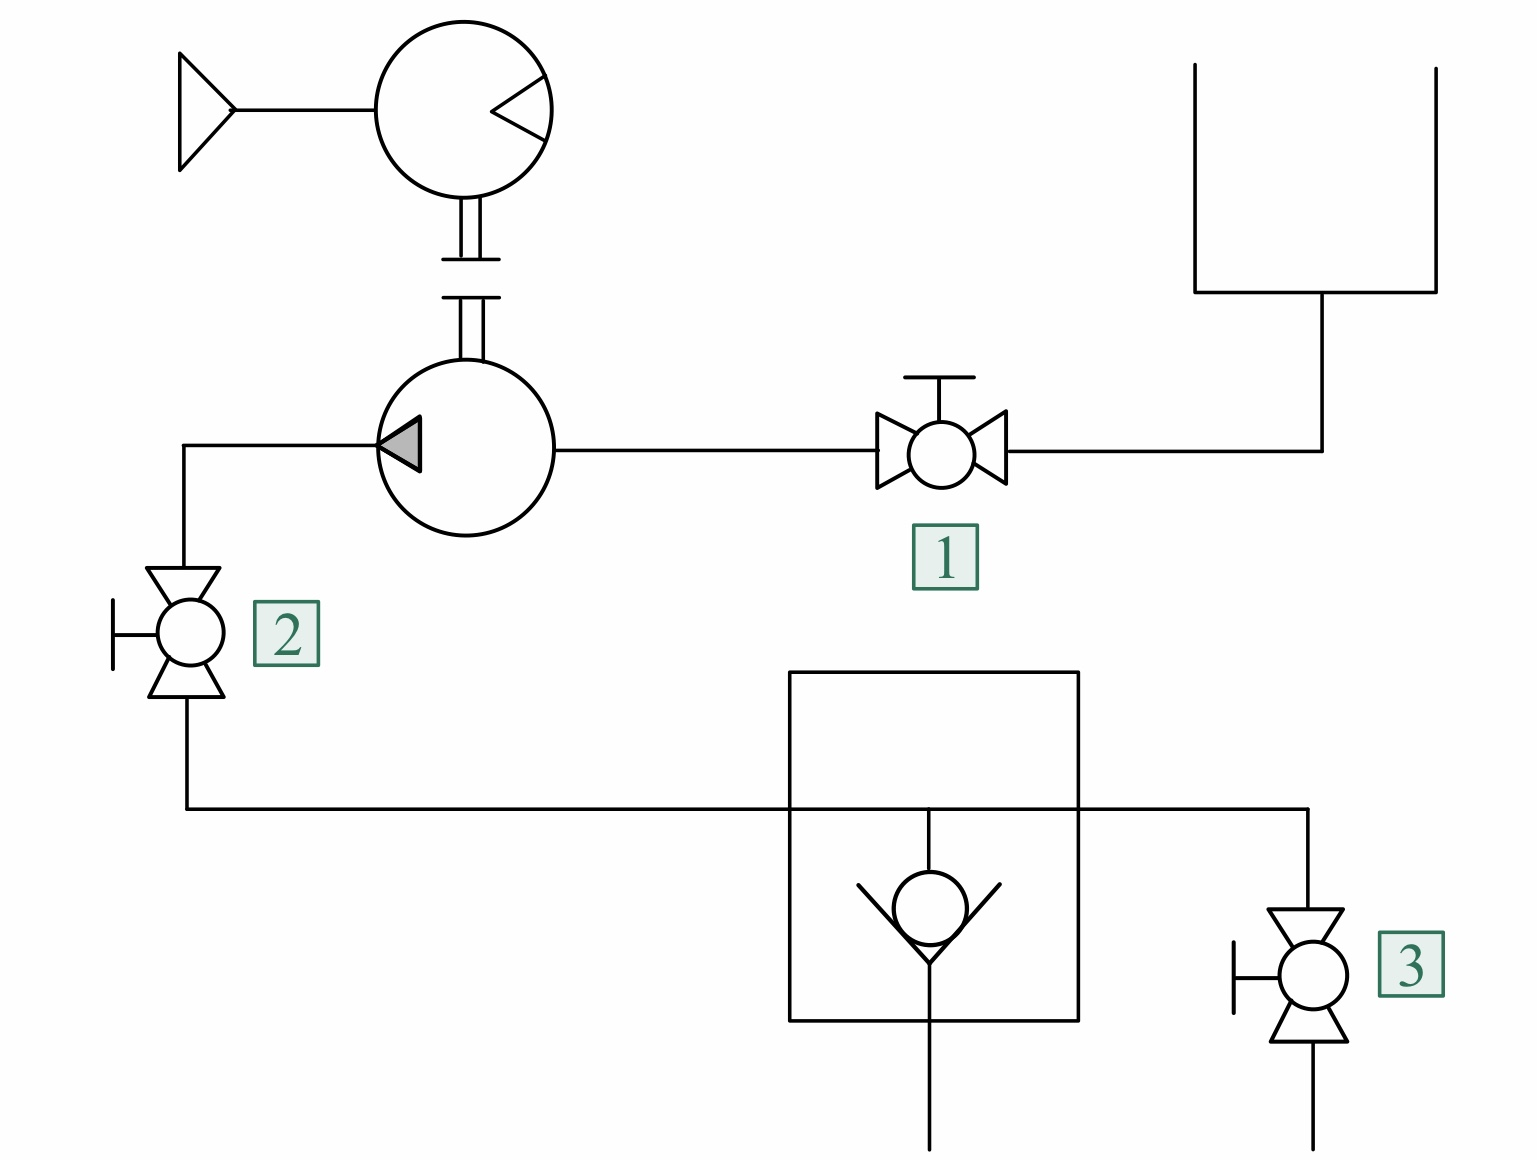
\includegraphics[width=0.45\textwidth]{figures/TestRig/oldTestRig.jpg}
    \caption{Sketch of a original available test rig.}
    \label{fig:oldTestRig}
\end{figure}


%%%%%%% Ball seat valve
Only the most fundamental components of the ball seat valve that play a critical role in its sealing 
are going to be covered in this article. The ball seat valve analyzed in the work, which is depicted 
in Fig.\Ref{fig:ballseatvalve}, is made up of a ball with a radius of 20 millimeters and a seat that has an
inner radius of 7.5 millimeters and a slope angle of 45 degrees. 
Both of these components are made of stainless steel.\\

\begin{figure}[htbp]
    \centering
    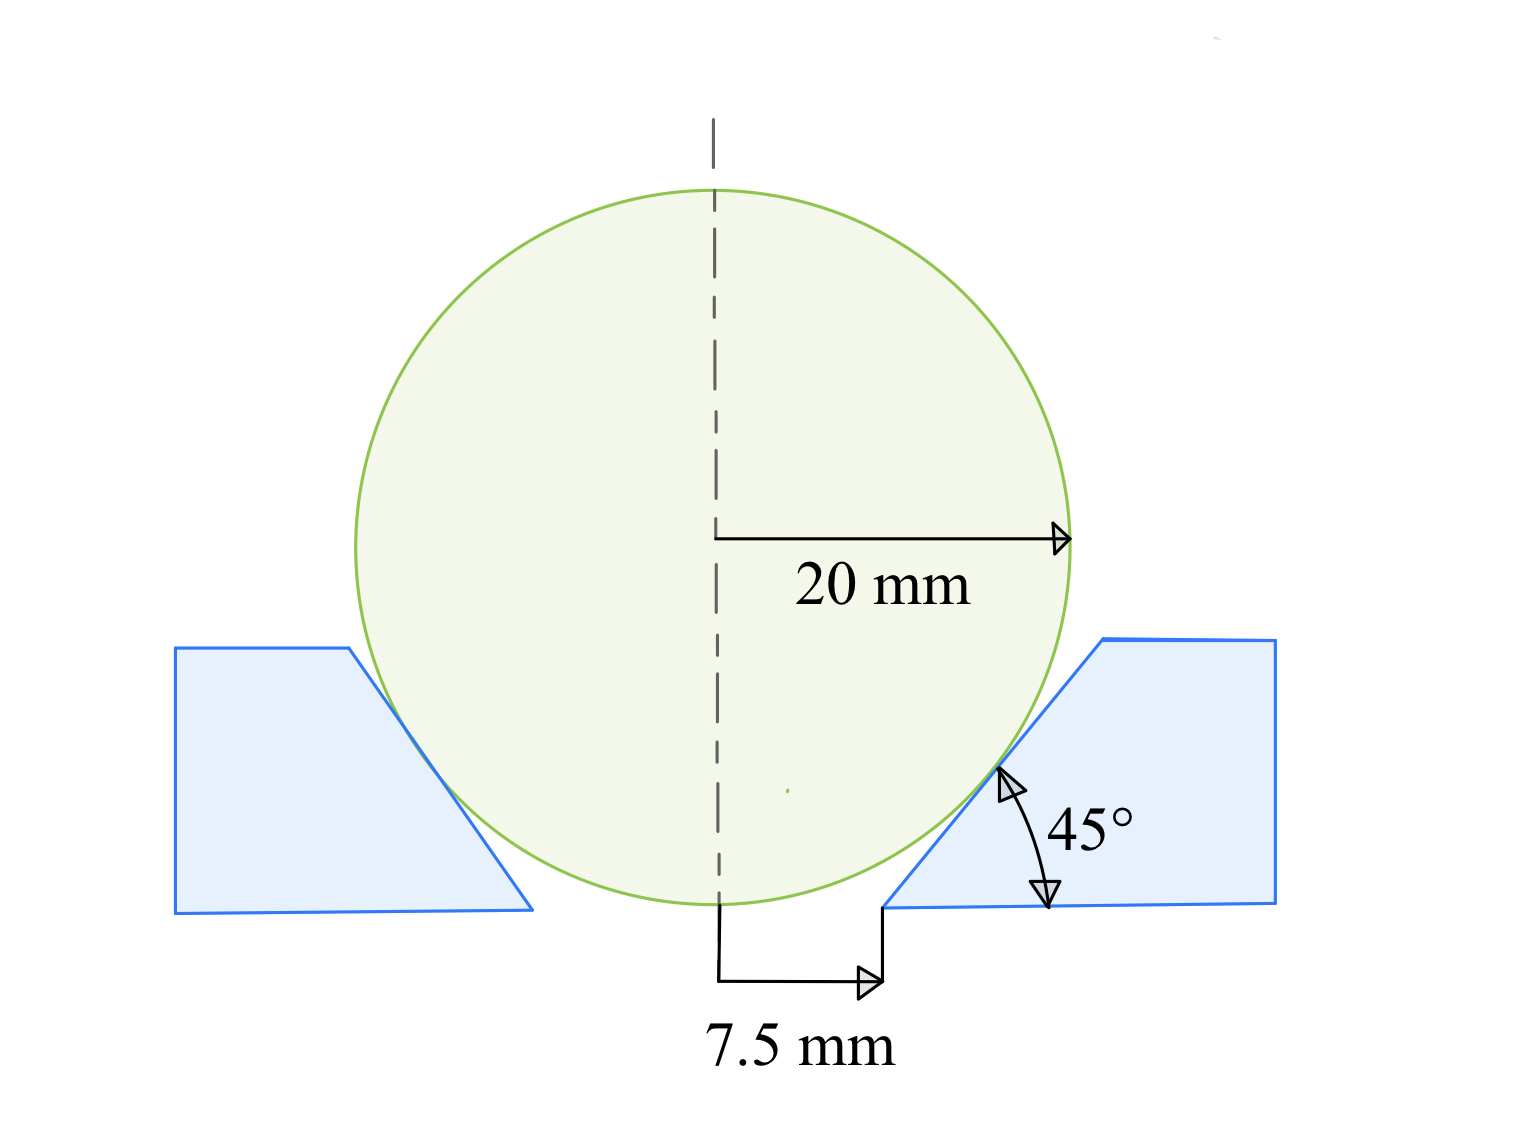
\includegraphics[width=0.45\textwidth]{figures/BallSeatValve/ballseatvalve.jpg}
    \caption{Sketch of ball seat valve.}
    \label{fig:ballseatvalve}
\end{figure}


The medium passing through the pipeline consists of distilled water and various types of microscopic particles. Distilled water
was chosen for two primary reasons. First, it comprises a negligible amount of particles,
which has the least potential impact on the particles being analyzed and reduces the 
errors caused in the test results. Also, water has a smaller viscosity as compared to
hydraulic oil, which is usually used in industrial applications. 
The smaller viscosity leads to a higher leakage, which is easier to measure \cite{fischer2021influence}.\\


Distilled water and particles will be mixed in a specific proportion. 
Through the water tank, the mixture is pumped into the pipeline, where 
it is transformed into a hydraulic medium and delivered on to the valve. 
Due to the imperfect sealing of the ball seat valve, distilled water can leak 
from a high-pressure environment to a low-pressure environment, i.e., to the 
atmosphere where the pressure is defined to be zero. This facilitates the detection of leaks, 
and the sealing of the ball seat valve can be analyzed by measuring the amount of leakage.\\

%%%%% problem of original test rig
The initial testing platform will be upgraded in order to keep the distilled water and microscopic
particles in the pipeline as uniformly mixed as feasible. As illustrated in Figure \Ref{fig:oldTestRig}, 
the medium 
entering the pipe from the tank either leaks into the atmosphere through the valve or flows out as 
wastewater at the end of the experiment through the opened drain ball valve No. 3 at the pipe's end, 
indicating that the pipe is not a closed circuit. During the process of measuring the leakage of the 
ball seat valve, the No. 3 drain valve always remains closed. When the sealing of the ball seat valve 
is not particularly poor, the amount of leaking fluid will be small, resulting in the mixture entering 
the pipe only being dynamic when it is just flowing into the pipe. As the mixture fills the pipe, its 
state gradually becomes static, which is likely to cause tiny particles to settle downwards due to their
own weight, thus accumulating in the pipe and failing to mix evenly with the distilled water, resulting 
in the actual concentration of particles in the mixture passing through the ball seat valve 
deviating too greatly from the initial set concentration added to the water tank. 

\begin{figure}[htbp]
    \centering
    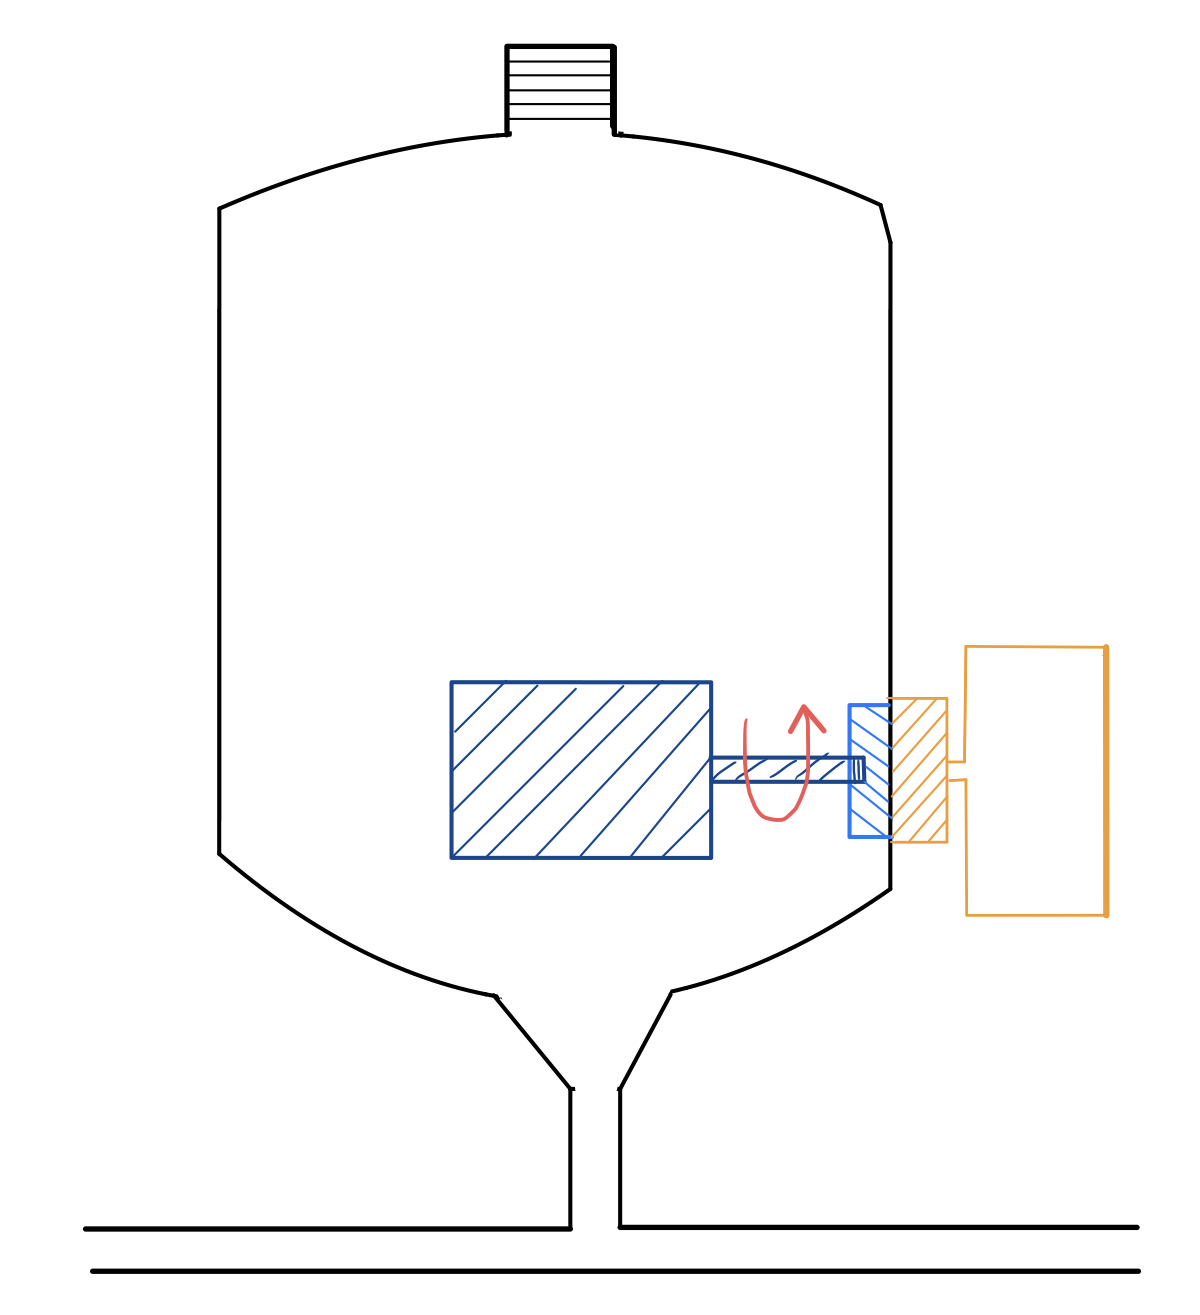
\includegraphics[width=0.34\textwidth]{figures/TestRig/Update1.jpg}
    \caption{Sketch of method 1 for improving the test rig. The water tank and pipes are in black colored,
     the stirrer is in dark blue colored, the internal magnet is in light blue colored and the external handle
      with magnet is in orange colored.}
    \label{fig:Update1}
\end{figure}



%%%%%% Update method 1
To avoid the issue described above, three methods have been tried to improve the test rig. The first 
approach is depicted in  Figure \Ref{fig:Update1}: a stirrer is placed in the water tank, and a magnet enables it to
be connected to an external magnetic handle across the tank's wall. The stirrer is then rotated by 
turning this external handle manually, allowing the particles and distilled water to mix uniformly.
However, there are two considerations with this method: first, how to place a stirrer with large 
enough blades inside a tank with a 31-cm-diameter entrance; and second, the manual turning of the 
handle is too slow to achieve homogenous mixing. Therefore this improvement is not considered.\\


%%%%%% Update method 2
The second approach envisaged is depicted in Figure \Ref{fig:Update2}; a small water pump is connected to the side of 
the tank in order to increase the energy of the mixing solution in the tank, thereby achieving a more
effective mixing effect. As the existing small pump has a maximum suction pressure of only 7 m of water 
column, which corresponds to approximately 0.7 bar, the suction side cannot be connected to the high 
pressure side. So this method is also not suitable.\\

\begin{figure}[htbp]
    \centering
    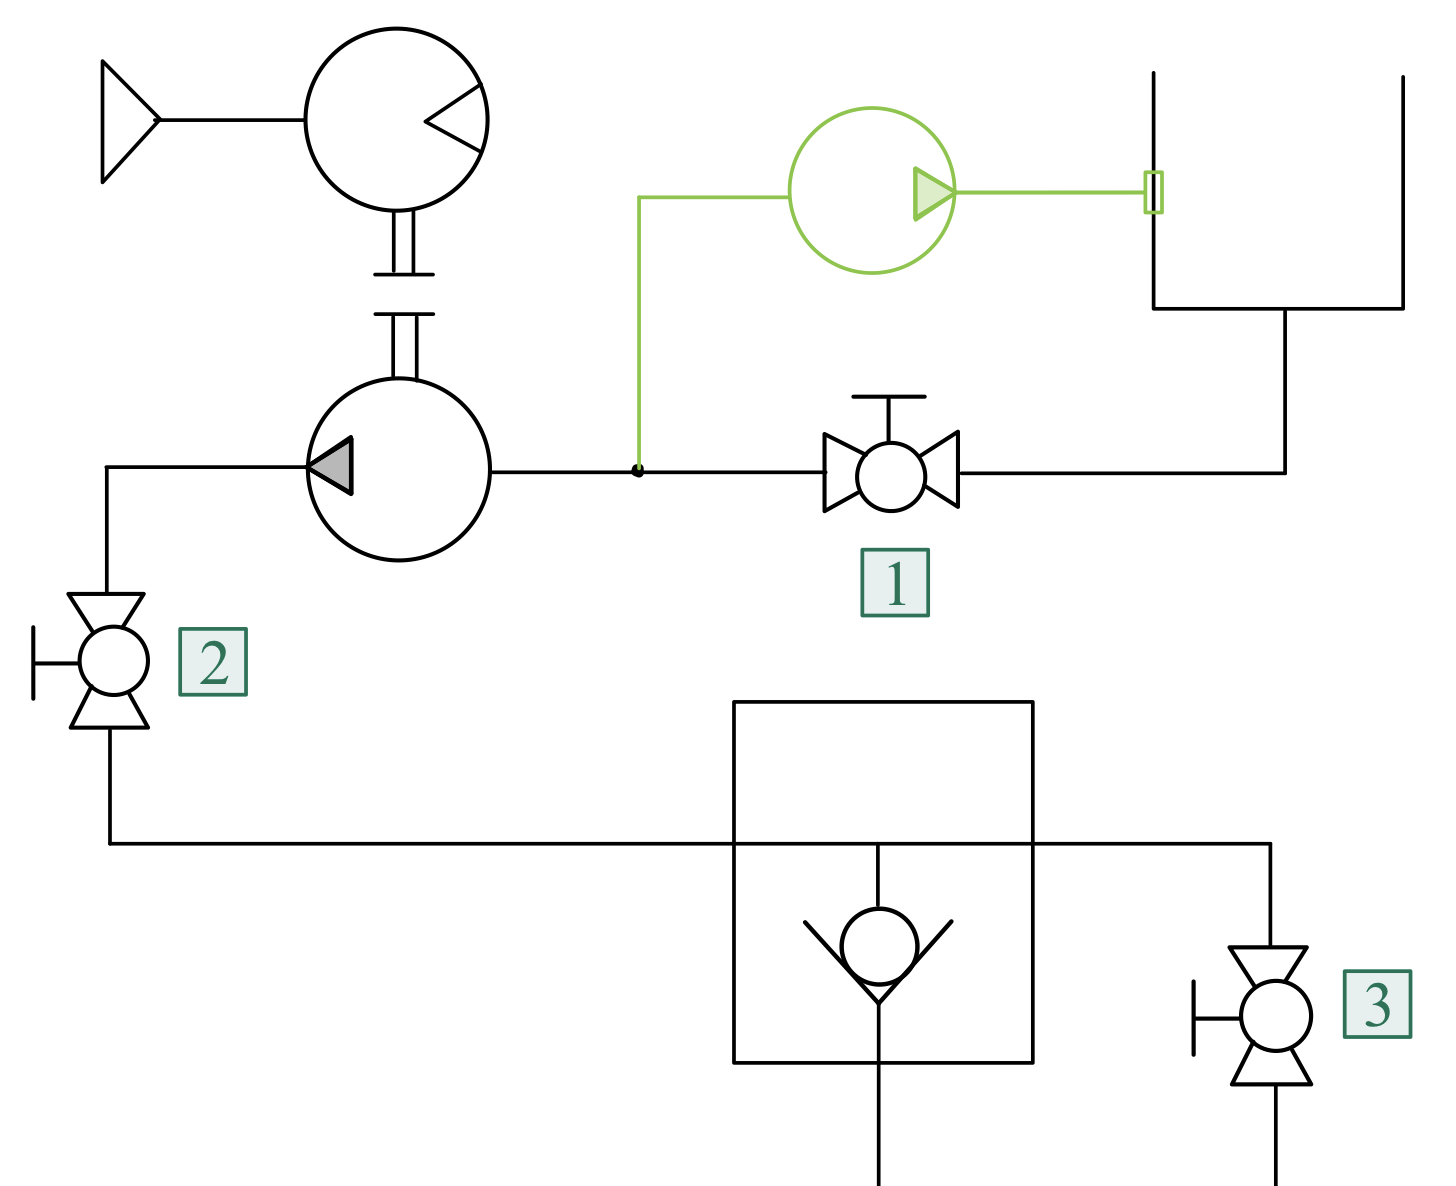
\includegraphics[width=0.43\textwidth]{figures/TestRig/Update2.jpg}
    \caption{Sketch of method 2 for improving the test rig. The small added water pump and pipes are in 
    green colored.}
    \label{fig:Update2}
\end{figure}

%%%%%% Update method 3
Finally, the test rig was improved by connecting the end of the original pipe to the tank with a new section of
pipe and a new ball valve No. 4, as illustrated in Figure \Ref{fig:newTestRig}. With the ball valve No. 4 partially open, 
the entire pipe forms a closed circuit, and the mixture is able to circulate through the pipe under 
the action of the hydraulic pump. The microscopic particles also gain more kinetic energy, decreasing 
the probability of deposition in the pipe and thus increasing the degree of mixing with distilled water. 
Special consideration should also be given to the fact that the ball valve No. 4 should only be partially 
opened and not entirely opened; otherwise, it will be challenging for the hydraulic system 
to attain and maintain the desired pressure level, it looks like a resistor or orifice.

\begin{figure}[H]
    \centering
    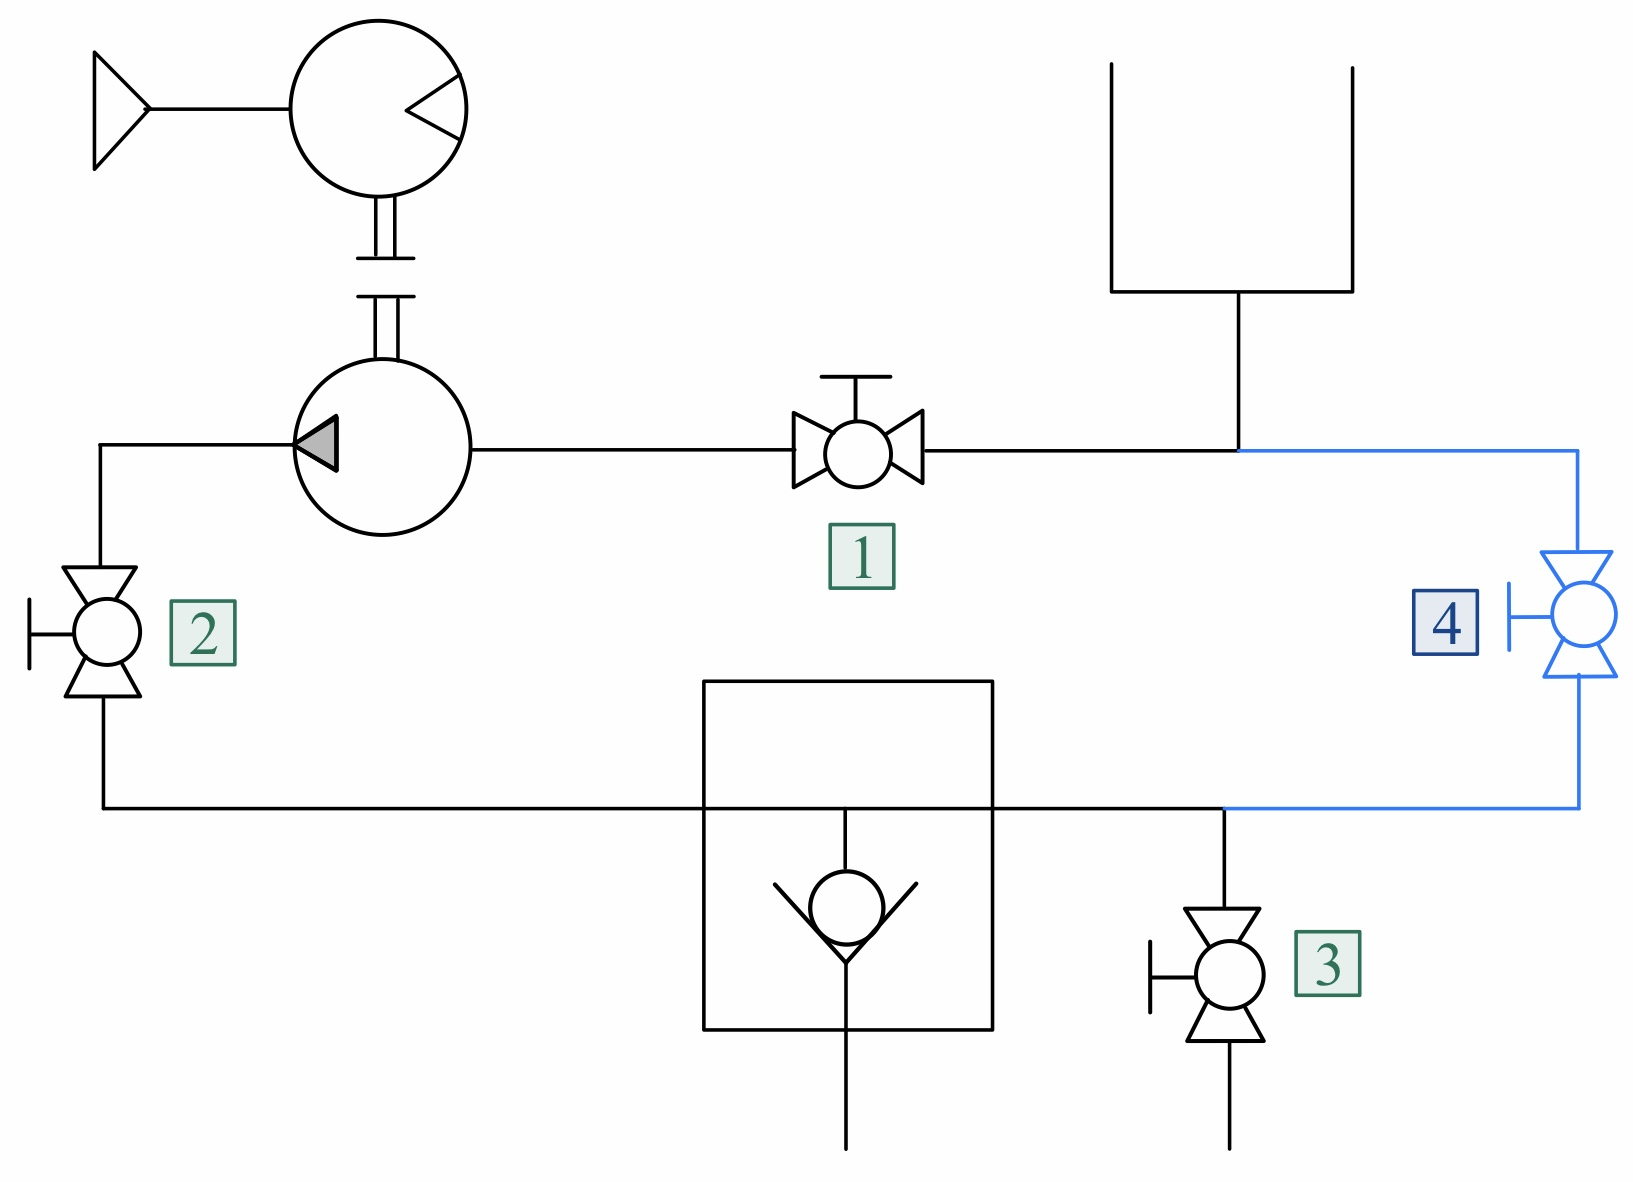
\includegraphics[width=0.45\textwidth]{figures/TestRig/newTestRig.jpg}
    \caption{Sketch of a improved test rig.}
    \label{fig:newTestRig}
\end{figure}

%%%%%%%%%%%%%%%%%%%%%%%%%%% new section: Qualification
\section{Qualification}
\label{Qualification}